\documentclass[11pt]{article}
\usepackage{amsmath,amssymb,amsthm}
\usepackage{fancyhdr}

% margins
\usepackage[vmargin=1in,hmargin=1.5in]{geometry}

% Drawing for Kmaps
\usepackage{tikz}
\usetikzlibrary{calc}
\usetikzlibrary{positioning}
\usetikzlibrary{matrix}
\pgfdeclarelayer{background}
\pgfsetlayers{background,main}

% Config
%%%%%%%%%%%%%%%%%%%%%%%%%%%%%%%%%%%
\newcommand{\lab}{4}
\newcommand{\name}{Connor Taffe}
\newcommand{\tno}{3742} % last 4 digits of T number.
%%%%%%%%%%%%%%%%%%%%%%%%%%%%%%%%%%%

\title{
	$L_{\lab}$ \\
	{\large Laboratory \rom{\lab}} \\
	{\normalsize Prof. Dr. P. Tang, CS 3482: Comp. Org. I}
}
\author{
	\name, T no. \tno
}

% TODO: Remember to update this.
\date{April $21^{\text{st}}$, 2015}

\pagestyle{fancy}
\rhead{Homework {\rom{\hw}}}
\lhead{{\name}. T no. \tno}

\usepackage{hw}

\begin{document}
\maketitle

\section{Details of Lab 4}

\begin{question}

	Here follows the Karnaugh map of $f$. \[f(a,b,c,d) = (a'+b)'c+d(b'+ac)\]

	\begin{figure}[h]
		\begin{center}
			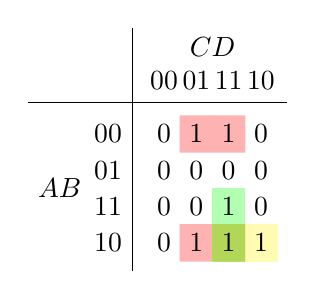
\begin{tikzpicture}
				\matrix (karnaugh) [matrix of math nodes] {
					0 & 1 & 1 & 0 \\
					0 & 0 & 0 & 0 \\
					0 & 0 & 1 & 0 \\
					0 & 1 & 1 & 1 \\
				};

				\foreach \i/\bits in {1/00,2/01,3/11,4/10} {
					\node [left  = 2mm of karnaugh-\i-1] {$\bits$};
					\node [above = 2mm of karnaugh-1-\i] {$\bits$};
				}

				\node [left  = .6cm of karnaugh.west]  (AB) {$AB$};
				\node [above = .5cm of karnaugh.north] (CD) {$CD$};

				\draw	($(CD.north -| karnaugh.west)  + (-.75mm,0)$)
						-- ($(karnaugh.south -| karnaugh.west)  + (-.75mm,0)$)
						($(AB.west |- karnaugh.north) + (0,+.40mm)$)
						-- ($(karnaugh.east |- karnaugh.north) + (0,+.40mm)$);

				\begin{pgfonlayer}{background}
					\begin{scope}[opacity=.3]
						\fill [red]
							(karnaugh-1-2.north west) rectangle (karnaugh-1-3.south east)
							(karnaugh-4-2.north west) rectangle (karnaugh-4-3.south east);
						\fill [yellow]
							(karnaugh-4-3.north west) rectangle (karnaugh-4-4.south east);
						\fill [green]
							(karnaugh-3-3.north west) rectangle (karnaugh-4-3.south east);
					\end{scope}
				\end{pgfonlayer}
			\end{tikzpicture}
		\end{center}
	\end{figure}

	Which shows that $f$ can be represented as the sum of minterms as follows: \[f(a,b,c,d)=b'd+acd+ab'c\]

\end{question}

\end{document}
